\documentclass[a4paper,8pt,openany]{book}
\usepackage[utf8]{inputenc}
\usepackage[french]{babel}
\usepackage[T1]{fontenc}
\usepackage{graphicx}
\usepackage{titlesec}
\usepackage{amsmath}
\usepackage{amsfonts}

\titleformat{\chapter}[block]
  {\normalfont\Huge\bfseries}% font of number
  {\chaptertitlename\ \thechapter~:}% format of number
  {20pt}% space between number and title
  {\Huge}% font of title

\titlespacing*{\chapter}
  {0pt}%  indent
  {0pt}% space before
  {20pt}% space after
\titlespacing*{\section}
  {0pt}%  indent
  {3.5ex plus 1ex minus .2ex}% space before
  {2.3ex plus .2ex}% space after

\author{Mendy Fatnassi}
\title{Cours de Mathematique sur les signaux}

%%%%%%%%%%%%%%%%%%%%%%%%%%%%%%%%%%%%%%	Page	%%%%%%%%%%%%%%%%%%%%%%%%%%%%%%%%%%%%%%%%
\begin{document}
\maketitle
\tableofcontents

\chapter{Nombre Complexe}

\section{Forme algebrique}

Les nombres complexe sont compris dans l'ensemble \mathbb{C} et il existe dans C un nombre i tel que $i^2 = -1$ .\\
Tout element de z dans C s'ecrit sous la forme $z=a+i.b$ avec a et b des reel.\\
- a est la partie Reel Re() \\
- b est la partie imaginaire Im() \\
\\
On peux pas avoir b=0 sinon cela veux dire que z=a donc z seras un reel .\\
\\
On peux representé cela graphiquement : \\

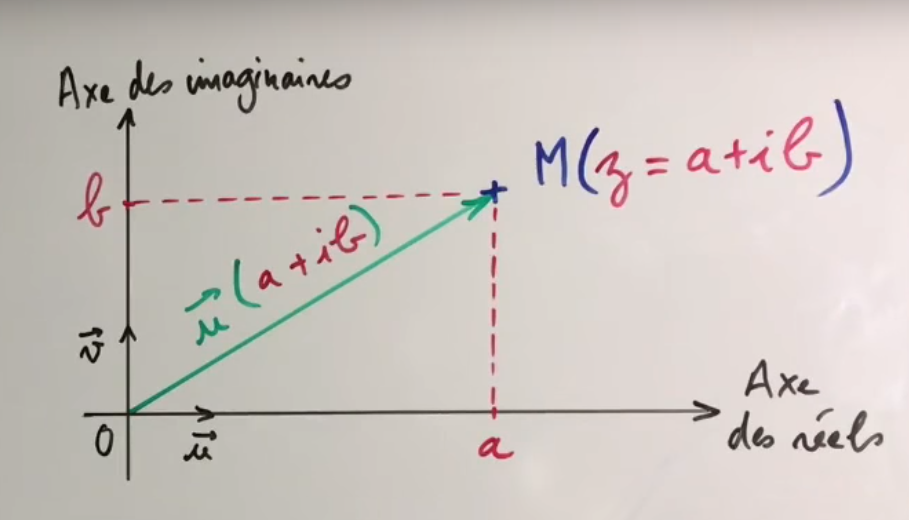
\includegraphics[width=0.5\textwidth , center]{img/NbComplexeAffixe.png}

le vecteur U pourras etre representer non plus par des coordonnes [a;b] mais par une seul formule , l'avantage seras de pouvoir faciliter certain calcule car on auras plus 2 nombre mais plus que 1 seul.\\ 

\section{conjuge}

Soit un nombre complexe z=a+ib , on appelle nombre \underline{complexe conjuge} de z le nombre z etoile z* = a-ib .\\

\section{Module et Argument}
\textbf{Module} :
\\
Le module correspond a la valeur absolue de z , il s'agit donc d'une longueur . \\
$|z|=sqrt(a^2+b^2)$ \\
\\
\textbf{Argument}
L'argument lui correspond a la valeur de l'angle $\theta$ .\\
$arg(z)=arctan - \frac{b}{a}$ \\
\\
\\
\\
\\
Graphiquement cela donne : \\
\\
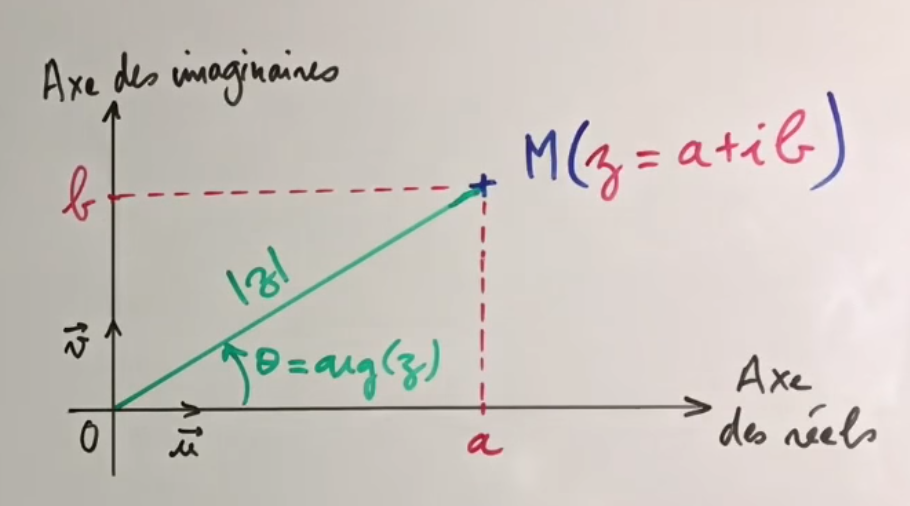
\includegraphics[width=0.5\textwidth , center]{img/NbComplexeArgMod.png}\\
\\

\section{Passage de formes}

\underline{Forme Algebrique} : \\
$z=a+ib$ \\
\\
\underline{Forme Exponentielle/Trigonometrique }\\
$z=|z|.e^{i.\theta}$ \\
sachant que $e^{i.\theta} =(cos(\theta) \time i.sin(\theta))$ \\
\\
\underline{propriete} : \\
$cos \theta - j.sin \theta = cos(- \theta)+j.sin(- \theta) = e^{-j \theta} = (e^{j \theta})* $\\






%%%%%%%%%%%%%%%%%%%%%%%%%%%%%%%%%%%%%%%%%%%%%%%%%SIGNAUX%%%%%%%%%%%%%%%%%%%%%%%%%%%%%%%%%%%%%%%%%%%%%%%%%
\chapter{Signaux}
Un signal peut etre representer par une fonction mathematique s qui peut dependre du temps , on aura donc s(t).\\
Un signal peut etre analogique ou numerique . Il est representé par une suite de nombre x[n].\\
\\
Signal analogique : t est continue t $\in$ dans R \\
Signal Numerique : t est discret , n $\in$ dans Z et x[n] est quantifié \\
\\
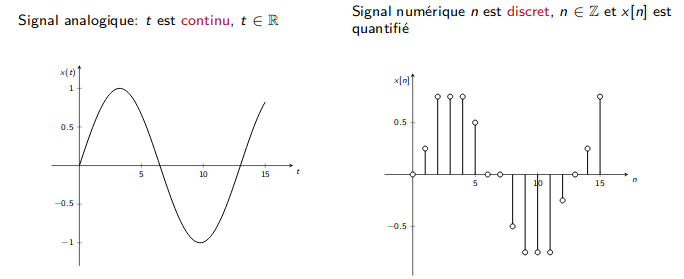
\includegraphics[width=1\textwidth,center]{img/signaux_anal_num.png}
\\
On peux representer un signal de facons temporelle (description analytique temporelle) ou frequentielle (representation spectrale).\\
\\
Voici ca representation \texbf{analytique temporelle} : \\
$s(t) = C + A sin(2\pi f0 t + \Phi )$  Avec \\
C : valeur de debut de l'abscisse ($\neq$ phase) , si on est centrée sur 0 ou une autre valeur de l'abscisse.\\
A : Amplitude Max .\\
f0 : frequence/nombre de repetiton .\\
$\Phi$ : Phase , Decallage du signal sur l'axe des abcisse par rapport a 0.\\

\section{Signaux Deterministe/Aleatoire}

\subsection{D\'eterministe}
Un signal d\'eterministe donne des valeurs identiques si on duplique la proc\'edure d’acquisition.\\
\\
Un signal d\'eterministe peut etre p\'eriodique/non-p\'eriodique : \\
Un signal d\'eterministe $s(t)$ est p\'eriodique de p\'eriode $T0$ si il v\'erifies $s(t)=s(t+T0)$.\\
Dans le cas contraire, le signal est non-p\'eriodique.\\
\\
La fr\'equence fondamentale F0 est l’inverse de la p\'eriode: $f0=\frac{1}{T0}$. \\
La periode fondamental s'obient donc par $T0=\frac{1}{f0}$ ,ou alors  $T0=\frac{temps_total}{nb_periode_total}$ avec f0:nb periode par sec\\
\\

\subsection{Aleatoire}

Un signal al\'eatoire est impr\'evisible: les valeurs ne se répètent pas a chaque mesure et l’on n’a pas de description analytique temporelle du signal.\\
Un signal al\'eatoire est soit stationnaire/non-stationnaire.\\
\\
\underline{Stationnaire} : Un signal est stationnaire si ses caractéristiques statistiques sont invariantes dans le temps (moyennes, variances).\\
\\
\underline{Non-stationnaire} : Un signal est non-stationnaire si ses caractéristiques statistiques évoluent dans le temps.\\

\textbf{Signaux theorique continue} : Ce sont des signaux qui n’existent pas dans la vraie vie. Ils ont les
caractéristiques suivantes:\\
-ils sont déterministes,\\
-ils sont définis par une fonction mathématique connue,\\
-on peut calculer facilement l’énergie et la puissance du signal.\\
\\
On a par exemple l'exponentiel ou la sinusoidale qui est un signal pure theorique.\\
Un signal theorique est different d'un signal reel qui lui contient du bruit (signal imparfait/pas lisse)\\

\chapter{Fonction Utile}

\textbf{Sin}\\
\underline{Formule} : $s(t)=C+ A sin(2\pi f0t + \Phi )$\\
\\

\textbf{Exponentiel}\\
\underline{Formule} : $s(t)=Ae^{-at}$\\
\\

\textbf{Fonction Echelon}\\
Elle se note $\Gamma$  \\
\\
\underline{Formule} :\\ 
$\Gamma$(t)= 0 si t < 0\\
          $= 1 si \geq 0 $\\
\\
\textbf{Fonction Rectangulaire} (ou Porte): \\
\underline{Formule} : $s(t)=A.rect(\frac{t}{a})$\\
Avec : A l'amplitude , $A=\frac{1}{a}$\\
t=Te , R\'ep\'eter l’op\'eration avec un d\'ecalage
temporel tout les t\\
a = Intervalle de temps ou l'on veux capturer le signal sur une duree tres courte a->0.\\
\\

\section{Amplitude d'un signal}

Un signal sinusoïdal est défini par une équation du type :\\
$s(t) = A sin(2\pi f0t + \Phi )$ avec :\\
\\
\\
\underline{L'amplitude}\\
L'amplitude repr\'esente la hauteur/l'intensit\'e du signal entre ces bornes min,max graphiquement le signal augmente sur l'axe des ordonn\'ee .\\
-A est appelé le gain ou bien l’amplitude maximum du signal\\
-A s’exprime dans l’unité de s ou bien en décibel: $A dB = 10 log(A)$\\
\\
\underline{La frequence} : \\
La frequence represente l'espacement du signal sur l'axe des abscisse , c'est cette frequence qui permet de produire des notes audible a certaine intervale de frequence .\\
La fréquence fondamentale f0 est l’inverse de la période: $f0=\frac{1}{T0}$ .La frequence peux aussi se trouver par  $f0=\frac{nb_periode_total}{temps_max}$\\
La periode fondamental s'obient donc par $T0=\frac{1}{f0}$ avec f0:nb periode par sec\\
\\
\underline{La phase} : \\
La phase représente le décalage à l’origine d’un signal , graphiquement cela donne une courbe qui commence pas sur l'axe 0 des abscisse, au lieu de commencer notre sinusoide par exemple a (0,0) , il commencera en (0,3) .Le signal debutera plus haut sur l'axe de l'ordonn\'ee a l'origine.
-\Phi est appelé la phase, elle est généralement donnée en radians\\
\\

\textbf{Signaux reel} : 
La frequence est exprim\'e en Hertz (Hz) \\
-Les signaux réels contiennent du bruit , on dit qu'il sont multi-fr\'equences.\\
-Ils possèdent plusieurs fréquences (cf séries de Fourrier).\\
-La fréquence fondamentale est la fréquence la plus basse.\\

\section{Energie et Puissance d'un signal deterministe}
\textbf{L'energie} est donn\'ee en Joule (J) et se note : $E = \int_+\infty^-\infty s^2(t) \mathrm dt$\\
On peux l'exprimer entre deux instant t1 et t2 et $T=t2-t1$ la duréé entre ces deux instants.\\
\\
\textbf{La puissance} s'exprime en Watts(W),on utilise plus commun\'ement des valeurs en décibels (dB),
telle que $P_{dB} = 10 \times log_10 (PW)$ et se note : $P=\lim\limits_{T \rightarrow +\infty}\frac{1}{T}\int_{-T/2}^{T/2} s^2(t)dt$\\
Et entre t1 et t2 : $P=\frac{1}{T} \int_{t2}^{t1} s^2(t)dt=\frac{E}{T}$\\
\\

%%%%%INCLURE SCHEMA%%%%%%%

Si la fonction echelon est de type : $\Gamma(t \pm TO)$ alors on dit que la fonction possede du retard .\\
Pour $\Gamma(t - TO) \rightarrow $ On a un retard de +TO .\\
Pour $\Gamma(t + TO) \rightarrow $ On a un retard de -TO .\\


\chapter{Numerisation du signal}
Pour passer d'un signal analogique a un signal numerique , il faut d'abord echantillonner celui-ci et le quantifier.\\
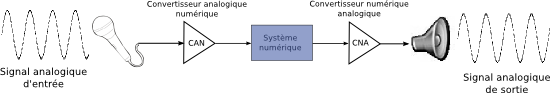
\includegraphics[width=1\textwidth,center]{img/enreg-numerique.png}\\
\\
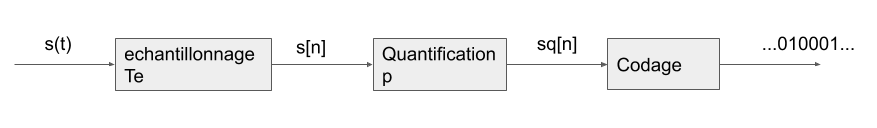
\includegraphics[width=1\textwidth,center]{img/chaine_numerisation_signal.png}\\
\\
\textbf{Echantillonage} :\\
On laisser passer le signal pendant une dur\'ee tr\'es courte $\delta$ t a intervalles de temps regulier Te.\\
Principe de l'interrupteur pour laisser passer la signal , cela se fait grace a la fonction rectangulaire $A.rect(\frac{t}{a})$\\
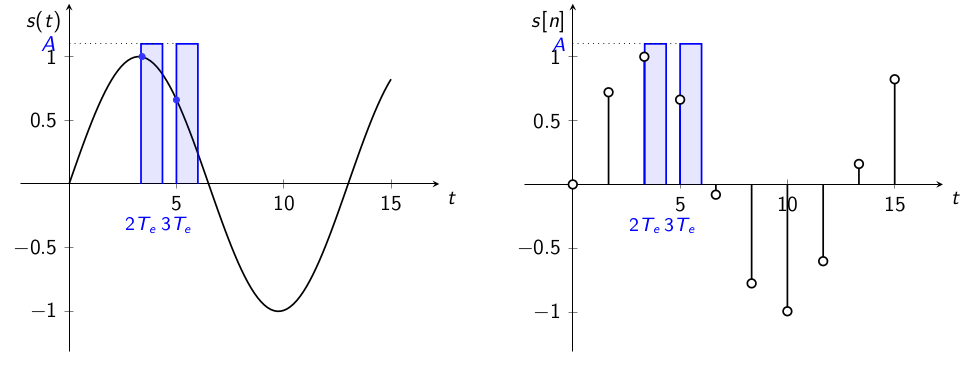
\includegraphics[width=0.75\textwidth,center]{img/echantillonage.png}\\
\\
La frequence d'echantillonage Fe se trouve comme pour une frequence normale $\times$ le nombre de point d'echantillonage $Fe=\frac{1}{T0}\times n$ avec n : nb point echantillonage.\\

\textbf{Quantification} :\\
 Les valeurs r\'eel $s(t)\in R$ ou s[n] sont discr\'etis\'e pour devenir des valeurs appartenant a un ensemble fini de valeurs possile.Plus on utilise de bits pour la quantification et plus elle seras pr\'ecise , on a donc $2^p$ pas de quantification avec p exprim\'e en bits. \\
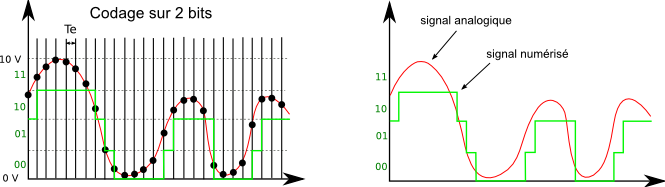
\includegraphics[width=1\textwidth,center]{img/quantification.png}\\
\\
Dans cet exemple, le signal a une amplitude de 10 volts :\\
0 à 2,5 V, le code sera « 00 »\\
2,5 V à 5 V, le code sera « 01 »\\
5 V à 7,5 V, le code sera « 10 »\\
7,5 V à 10 V, le code sera « 11 »\\
\\


\chapter{Dirac}
La distribution de Dirac, aussi appelée par abus de langage fonction $\delta$ de Dirac, peut être informellement considérée comme une fonction qui prend une « valeur » infinie en 0, et la valeur zéro partout ailleurs, et dont l'intégrale sur R est égale à 1. on a donc $\delta = +\infty$ si t=0 sinon 0.\\
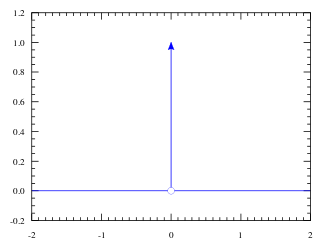
\includegraphics[width=0.60\textwidth,center]{img/dirac.png}
\\
Il peux servir a calculer une impulsion de dirac.L'integrale d'un dirac est egale a 1 $\int_{+\infty}^{-\infty} \delta(t) \mathrm dt = 1$.\\
Un dirac commence a $\delta(t)$  on peux aussi deplacer cette variable ailleur en t0 , $\delta(t-t0)$\\
\\


\section{Peigne de dirac}
Un peigne de dirac est une somme de distributions de Dirac espacées de T.Cette distribution périodique est particulièrement utile dans les problèmes d'échantillonnage, remplacement d'une fonction continue par une suite de valeurs de la fonction séparées par un pas de temps T.\\
On peux developper cette fonction en serie de fourrier.\\
\\
\underline{Formule Peigne Dirac} :\\
$III_{Te}\sum_{-\infty}^{+\infty} \delta(t-n.Te)$ (faut que n>0)\\
$III_{Te}(t)= \delta(t)+\delta(t-Te)+\delta(t-2Te)+...+\delta(t-nTe)$\\
\\
Le peigne dirac peux servir a l'echantillonage d'un signal par exemple en multipliant le signal par un dirac , exemple :\\
on a un signal $s(t)=sin(2\pi f0t)$ et un dirac $\delta(t-Te)$ alors le fait de faire $s(t).\delta(t-Te)=s(Te).\delta(t-Te)$ nous permettra d'avoir des dirac qui serons non plus centr\'ee sur 1 mais sur le signal lui meme.\\
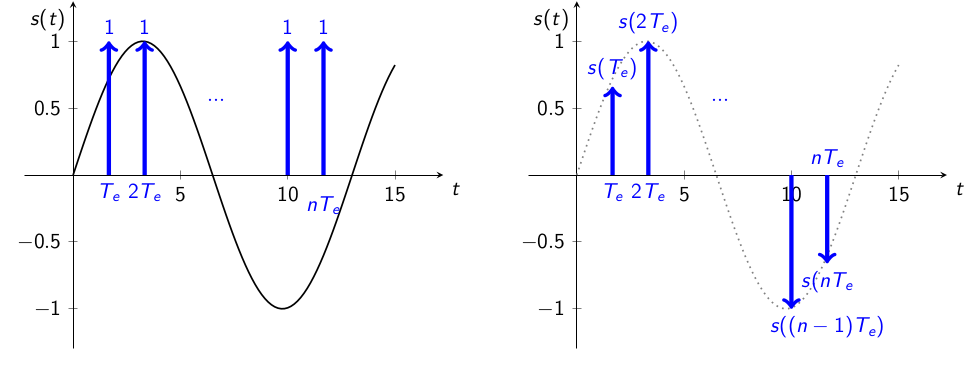
\includegraphics[width=0.60\textwidth,center]{img/peigne_dirac.png}

\chapter{Serie de Fourrier}
\section{Serie de Fourrier}
Un signal electrique re\'el peut se decomposer comme une somme de sin() et cos() c'est ce qu'on appelle la serie de fourrier , c'est aussi un signal multi-frequence .Cela s'applique seulement si le signal est periodique et continue.\\
\\
Sous certaines conditions de dérivation et de continuité, tout signal à temps continu s(t) périodiquede période T0 peut s’écrire sous la forme d’une somme de signaux sinusoïdaux.\\
Cette somme peut s’écrire de deux manières :\\
-1)forme trigonométrique réelle\\
-2)forme exponentielle complexe\\
\\
\underline{Formule Serie de Fourrier} :\\
1)$x(t)=a0+\sum_{n=1}^{+\infty}(an.cos((2\pi fo.t)+bn sin(2\pi fot)$\\
Avec : \\
-a0 qui correspond a la valeur moyenne (composante continue): $a0=\frac{1}{T0}\int_T0^0 x(t) \, \mathrm dt$\\
-an et bn sont les coef. de la serie de fourrier : $an=\frac{2}{T0}\int_T0^0 x(t)cos(2\pi f0.n.t) \, \mathrm dt$\\
et $bn=\frac{2}{T0}\int_T0^0 x(t)sin(2\pi f0.n.t) \, \mathrm dt$\\
avec f0.n qu'on appelle frequence harmonique.\\
\\
La serie de fourrier peux s'ecrire de facons plus condens\'e (Developpement Harmonique):
$x(t)=a0+\sum_{n=1}^{+\infty}Cn cos(2\pi f0.t+\Phi n)$\\
Avec : $Cn=\sqrt{an^2+bn^2}$ et $\Phi n=arctan(-\frac{bn}{an}$\\
\\
2)$x(t)=\sum_{-\infty}^{+\infty} Sn e^{j2\pi nf0t}$\\
$Sn=\frac{1}{T0}\int_0^{T0} x(t) e^{j2\pi f0nt} dt\\

\section{Transform\'ee de Fourrier }
La serie de fourrier s'applique dans le domaine discret periodique de T0 , La Transform\'ee de fourrier appartient au domaine continue et se note : \\
$X(f)=\int_{-\infty}^{+\infty} x(t) e^{-j2\pi ft} dt$\\
\\
La transformée de Fourier est un opérateur mathématique qui:\\
-ne modifie pas le signal x (t)\\
-permet d’analyser et de représenter le signal x dans le domaine fr\'equentiel\\



\end{document}